Studying the dynamics of solid-state systems far from equilibrium with ultrafast experimental techniques has gained attraction over the last decades.
These techniques allow to probe different observables on femtosecond timescales, shedding light on the relaxation pathways towards equilibrium.

\textbf{pump-probe}

A simple concept to reach high time resolutions is the pump-prope technique.
The basic idea is that an excitation event (pump) and a probe event with a known variable time difference occur on the sample under investigation.
The excitation event may be an arriving optical laser pulse and the probe event might be the scattering of an electron or X-ray pulse.
If probe-events are measured while continiously varying the time delay the data can be assembled into a \emph{movie}.
Both, excitation and probe event, are required to be shorter than the time scale of the pheonomenon under investigation.
If the phenomenon under study is reversable and there is enough time between each excitation event, a measurement can be done continiously on one sample.
Current plans do not involve studying irreversible phenomena.

\begin{figure}[!t]
	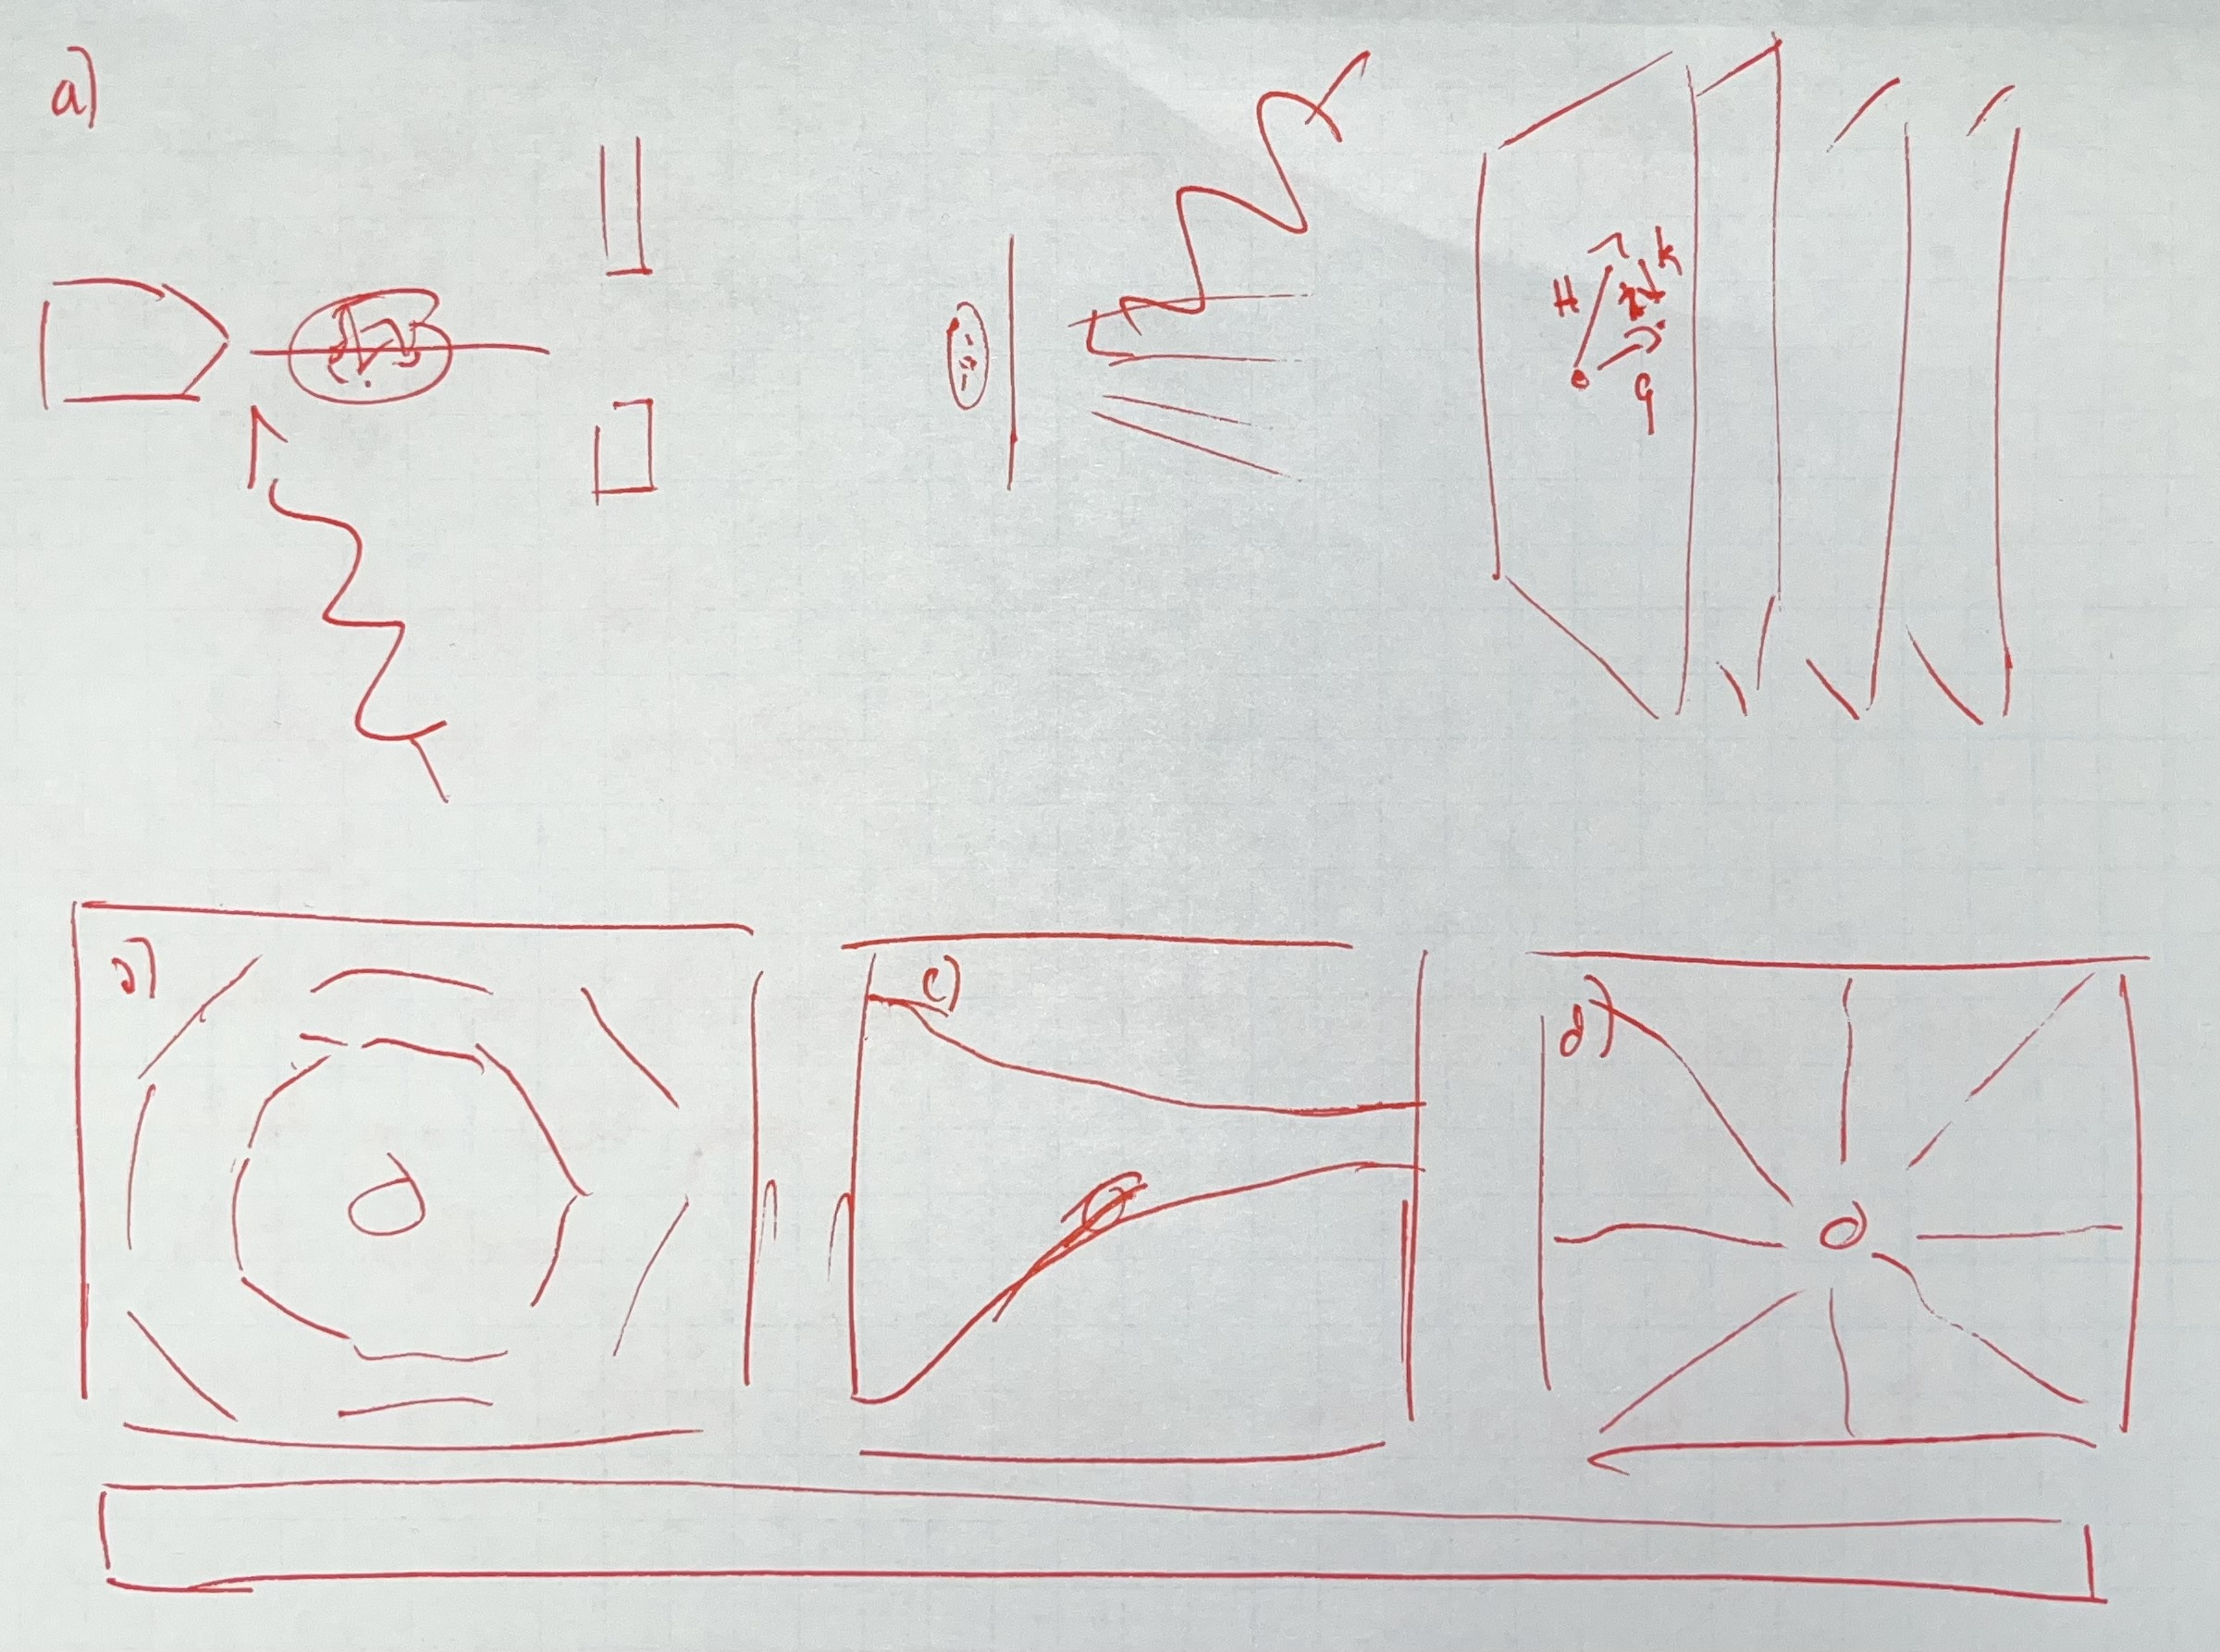
\includegraphics[width=\columnwidth]{figs/method_placeholder.jpg}
	\caption{\textbf{a)}\,Working principal of \acs{UEDS}. The laser pump pulse arrives at the sample, followed by the electron probe pulse with a time delay of $\tau$. The electrons are scattered off of the sample and collected on the detector. For one pixel on the detector the scattering vector $\mathbf{q}$, its reduced wave vector $\mathbf{k}$ and the closest Bragg reflection $\mathbf{H}$ are shown. One-phonon structure factors of the longitudinal (\textbf{b}) and transverse (\textbf{c}) acoustic modes in the high temperature phase of \ts.}
	\label{fig:method}
\end{figure}

\textbf{UED/UEDS}

Building on the idea of the pump-probe scheme one can combine classical electron diffraction experiments and femtosecond laser systems and conduct \ac{UED} and \ac{UEDS} experiments.

The experimental apparatus starts with a commercial Ti:sapphire laser system emitting $\sim$35\,fs laser pulses with a center wavelength of 800\,nm, that are split and guided onto different beam path.
For sample excitation one part of the pulse is attenuated and guided onto the sample.
Part of the pulse entering the probe beam path is frequency doubled. The fundamental and frequency doubled pulses are converted to a pulse with a center wavelength of 266\,nm by frequency summation.
The final pulse is guided onto a photo cathode in vacuum, where the electron bunch that will be scattered from the sample is being created.
The electron bunch is accelerated to 90\,keV by a static electric field and focused onto the sample.
On its way to the sample the electron bunch will broaden considerably due to Coulomb repulsion, effectively limiting the time resolution of the experiments.
To compensate for this effect the electron bunches are re-compressed in a radio-frequency driven cavity between the electron gun and the sample.
A schematic representation is shown in shown in figure~\ref{fig:method}\,a:
Laser pump and electron probe pulse arrive at the sample with a time delay of $\tau$.
The scattering patterns are collected in a transmission geometry and varying the time delay allows to capture dynamics of the studied system.

The datasets collected are incredibly rich and contain information about wave-vector-dependent dynamics of the phonon system across the whole \ac{BZ}.
The total scattering intensity collected on the detector is in the kinematic approximation
\begin{equation} I(\mathbf{q},t) = \sum_n I_n(\mathbf{q},t)\enspace\text{with}\enspace n \in\mathbb{N},\label{eq:I}\end{equation}
with the scattered intensities $I_n$ of an electron that scattered with $n$ phonons at scattering vector $\mathbf{q}$ at time $t$.
The contribution the the scattered intensity decreases rapidly for higher order terms, hence only the first two terms will be discussed.

The first term describes the intensity of the electrons diffraction into Bragg spots with the proportionality
\begin{equation} I_0(\mathbf{q}, t) \propto \left| \sum_s f_s(\mathbf{q}) \e^{-W_s(\mathbf{q},t)} \e^{-\i[\mathbf{q}\cdot\mathbf{R}_s(t)]} \right| ^2.\label{eq:I0}\end{equation}
the sum expression is the so called geometric structure factor and contains the atomic form factors $\{f_s(\mathbf{q})\}$ (determined by the scattering potential of each atomic species), the Debye-Waller factors $\{\e^{-W_s(\mathbf{q},t)}\}$ and phase factors $\{\e^{-\i[\mathbf{q}\cdot\mathbf{R}_s(t)]}\}$ with the atomic positions in the unit cell $\{\mathbf{R}_s(t)\}$, $s$ is running over the atoms in the unit cell.
The real space structure of the sample cannot be calculated from the diffraction, since the phase factor information is lost due to the absolute square.
Information about thermal motion of the atoms is encoded in the Debye-Waller factor.
It is proportional to the mean square atomic displacement of the atoms around their equilibrium position, thus containing information on all phonon modes.
The factor leads to an intensity reduction of the Bragg spots.

To track the phonon dynamics in more detail, namely in energy, momentum and time, one must also consider the intensity of scattering event involving a single phonon

\begin{equation} I_1(\mathbf{q},t) \propto \sum_i \frac{n_i(\mathbf{k})+\frac{1}{2}}{\omega_i(\mathbf{k})}\,\left| F_{1,i}(\mathbf{q},t) \right|^2 = \sum_i \frac{n_{i,\mathbf{k}}(t)+\frac{1}{2}}{\omega_{i,\mathbf{k}}(t)}\,\left| \sum_s \e^{-W_s(\mathbf{q},t)} \frac{f_s(\mathbf{q})}{\sqrt{\mu_s}} \left( \mathbf{q}\cdot\mathbf{e}_{i, s}(\mathbf{k}) \right) \right|^2.\label{eq:I1}\end{equation}
The index of the outer sum $i$ runs over all phonon modes populations $\{n_{i,\mathbf{k}}\}$ and their respective frequencies $\{\omega_{i,\mathbf{k}}\}$.
$\left| F_{1,i}(\mathbf{q},t) \right|^2$ is the one-phonon structure factor and weighs the contribution of each phonon mode $j$ to the first order diffuse scattering intensity.
In full the one-phonon structure factor is written on the RHS of equation~\ref{eq:I1} with index $s$ running over the atoms in the unit cell and the Debye-Waller and the atomic form factors from equation~\ref{eq:I0} and the atomic masses $\{\mu_s\}$ and the phononic polarization vectors $\{\mathbf{e}_{i, s}(\mathbf{k})\}$.

To track the flow of energy in the sample after optical excitation and access to the changes population dynamics across the \ac{BZ} is important.
In order to derive $\{n_{i,\mathbf{k}}\}(t))$ from the first-order diffuse scattering intensity, one must obtain knowledge of the one-phonon scattering factors and the phonon frequencies.
A extensive description on how to calculate the $\left| F_{1,i}(\mathbf{q},t) \right|^2$ and finally electron-phonon coupling constants is presented in~\cite{stern2018,renedecotret2019}.

In short: \Ac{DFT} calculations and clustering algorithms are used to obtain the polarization $\mathbf{e}_{i,s,\mathbf{k}}$ and frequency $\omega_{j,\mathbf{k}}$ of each phonon and sort them into branches.
Any transient changes in the Debye-Waller factor are negligible and therefore they can also be obtained from the polarizations determined by the \ac{DFT} calculation.
The evaluated phonon mode populations 
The calculations were carried out for the high temperature phase of \ts at room temperature and the result for the longitudinal/transverse acoustic mode is displayed in figure~\ref{fig:method}\,b/c.
Lets discuss the implications of the scalar product $\left( \mathbf{q}\cdot\mathbf{e}_{i, s}(\mathbf{k}) \right)$ in equation~\ref{eq:I1} on both of the structure factors.
For the transverse phonon mode the structure factor is large from $\Gamma$ along the azimuthal direction, because the mode polarization is perpendicular to $\mathbf{q}$.
Vice versa the structure factor of the longitudinal mode is parallel to $\mathbf{q}$ and exhibits prominent features radially.
With the frequencies and one-phonon structure factor on hand the derivation of the phonon populations $\{n_{i,\mathbf{k}}(t)\}$ is straightforward.
Employing the so called nonthermal lattice model\cite{waldecker2016} (a set of coupled equations, with a temperature and a heat capacity assigned to the electron system and each phonon mode) allows to determine electron-phonon coupling constants.

In 2021 Zacharias et~al. published methods to extend the presented calculation to multi-phonon structure factors of orders $n\geq 2$ (see equation~\ref{eq:I}).
Further they compare the theoretical results with experimental data on different 2D-materials, including \acp{TMD}, showing good agreement\cite{zacharias2021a,zacharias2021b}.

%capabilities of the machine
%epc
% photoexcitation absorbed by electrons
% electrons couple to phonons -> heat
%samples are easy to use
%peak width <-> correlation length
%multi-phonon structure calculation